%!TEX root = ../main.tex

\section{Implementation Details of Tree-Based Agentic Reasoning}
\label{sec:appendix_agentic_reasoning}

In this section, we provide the implementation details of the tree-based agentic reasoning mechanism described in Section~\ref{sec:tree_based_agentic_reasoning}, including prompt construction, schema handling, table content representation, state representation, failed branch reuse, and the algorithm pseudo-code.

\subsection{Prompt Construction}
\label{subsec:appendix_deepprep_prompt}

We present the detailed prompts of \sys. The prompt of \sys consists of an initial prompt and trajectory prompts that are incrementally updated during multi-turn interaction.

%!TEX root = ../../main.tex
\begin{figure}[!t]
    \centering 
    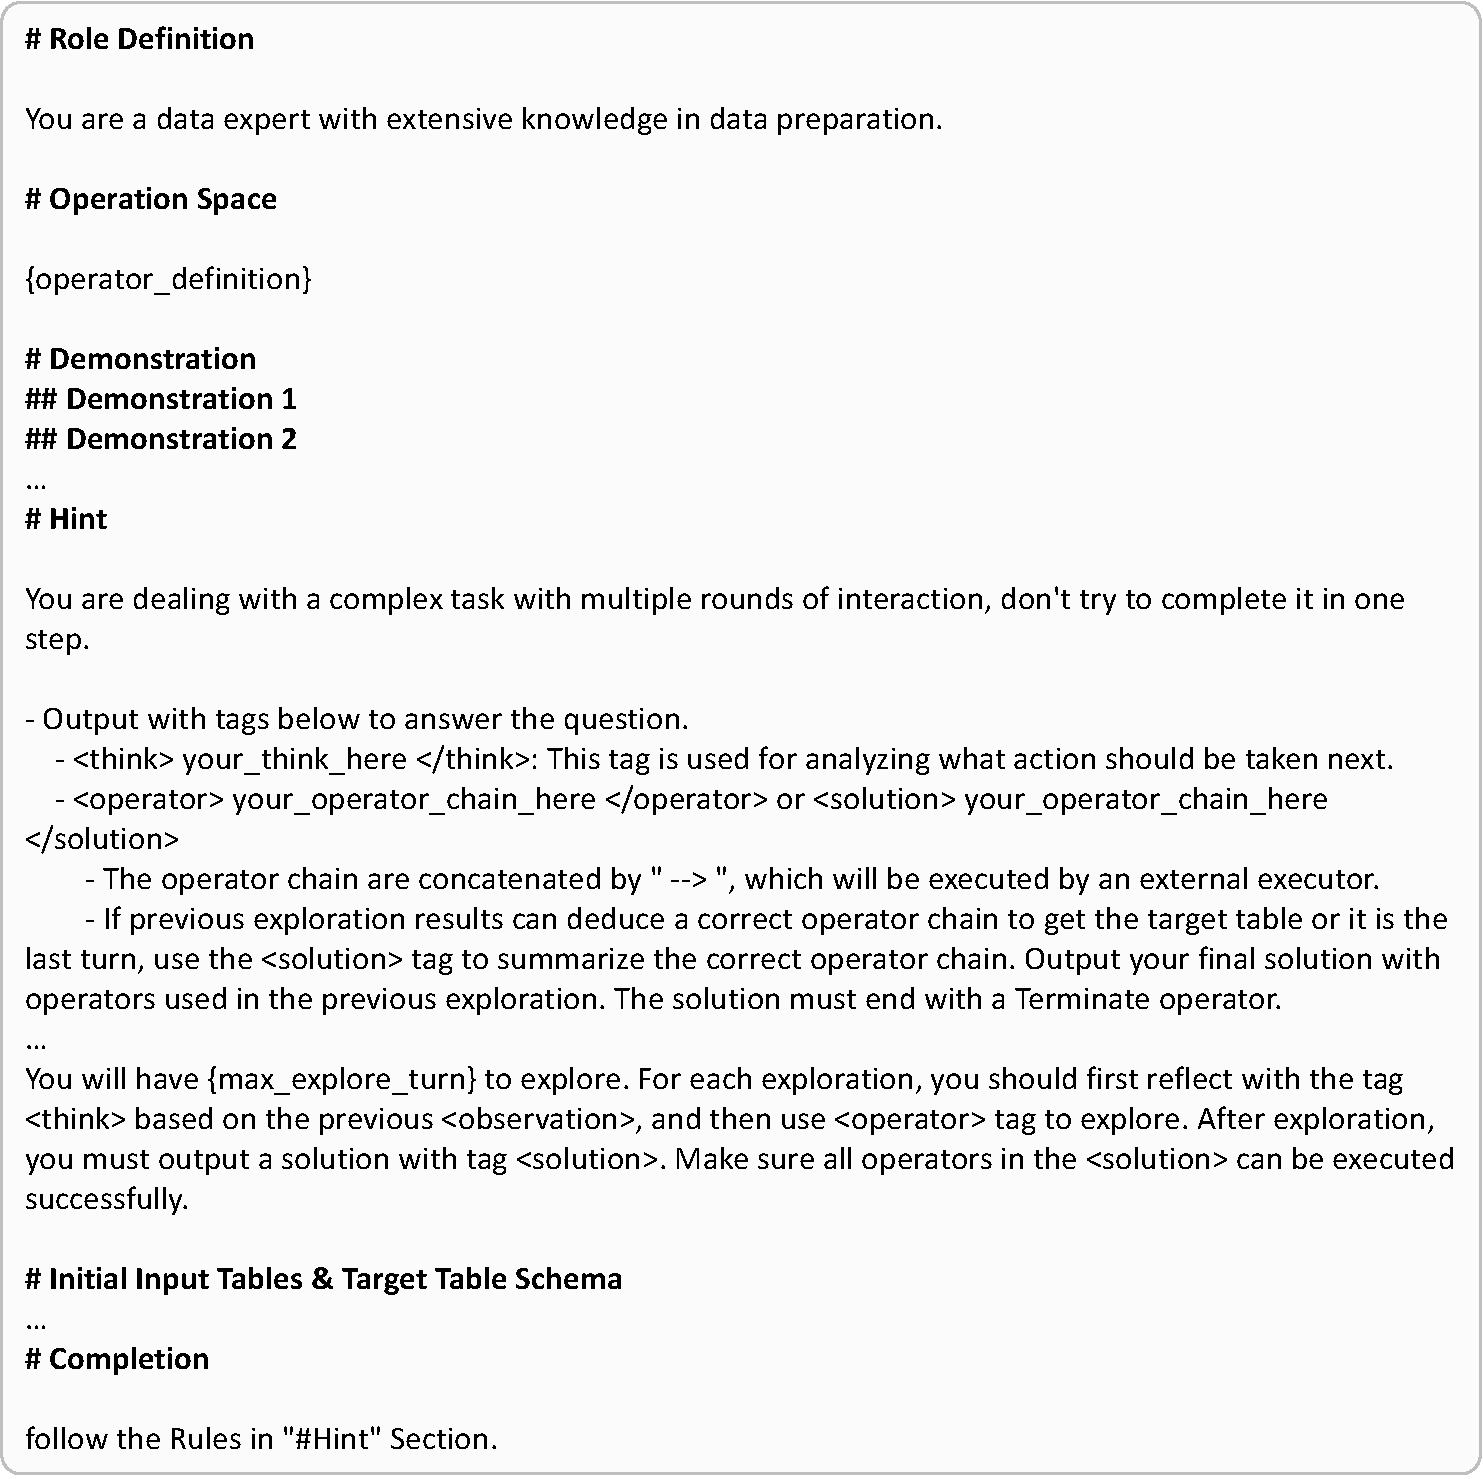
\includegraphics[width=1.01\columnwidth]{appendix/figures/fig/deepprep_initial_prompt.pdf}
    \vspace{-2em}
    \caption{Prompt of \sys.
    }
    \label{fig:deepprep_initial_prompt}
    \vspace{-1em}
\end{figure}

%!TEX root = ../../main.tex
\begin{figure*}[!t]
    \centering 
    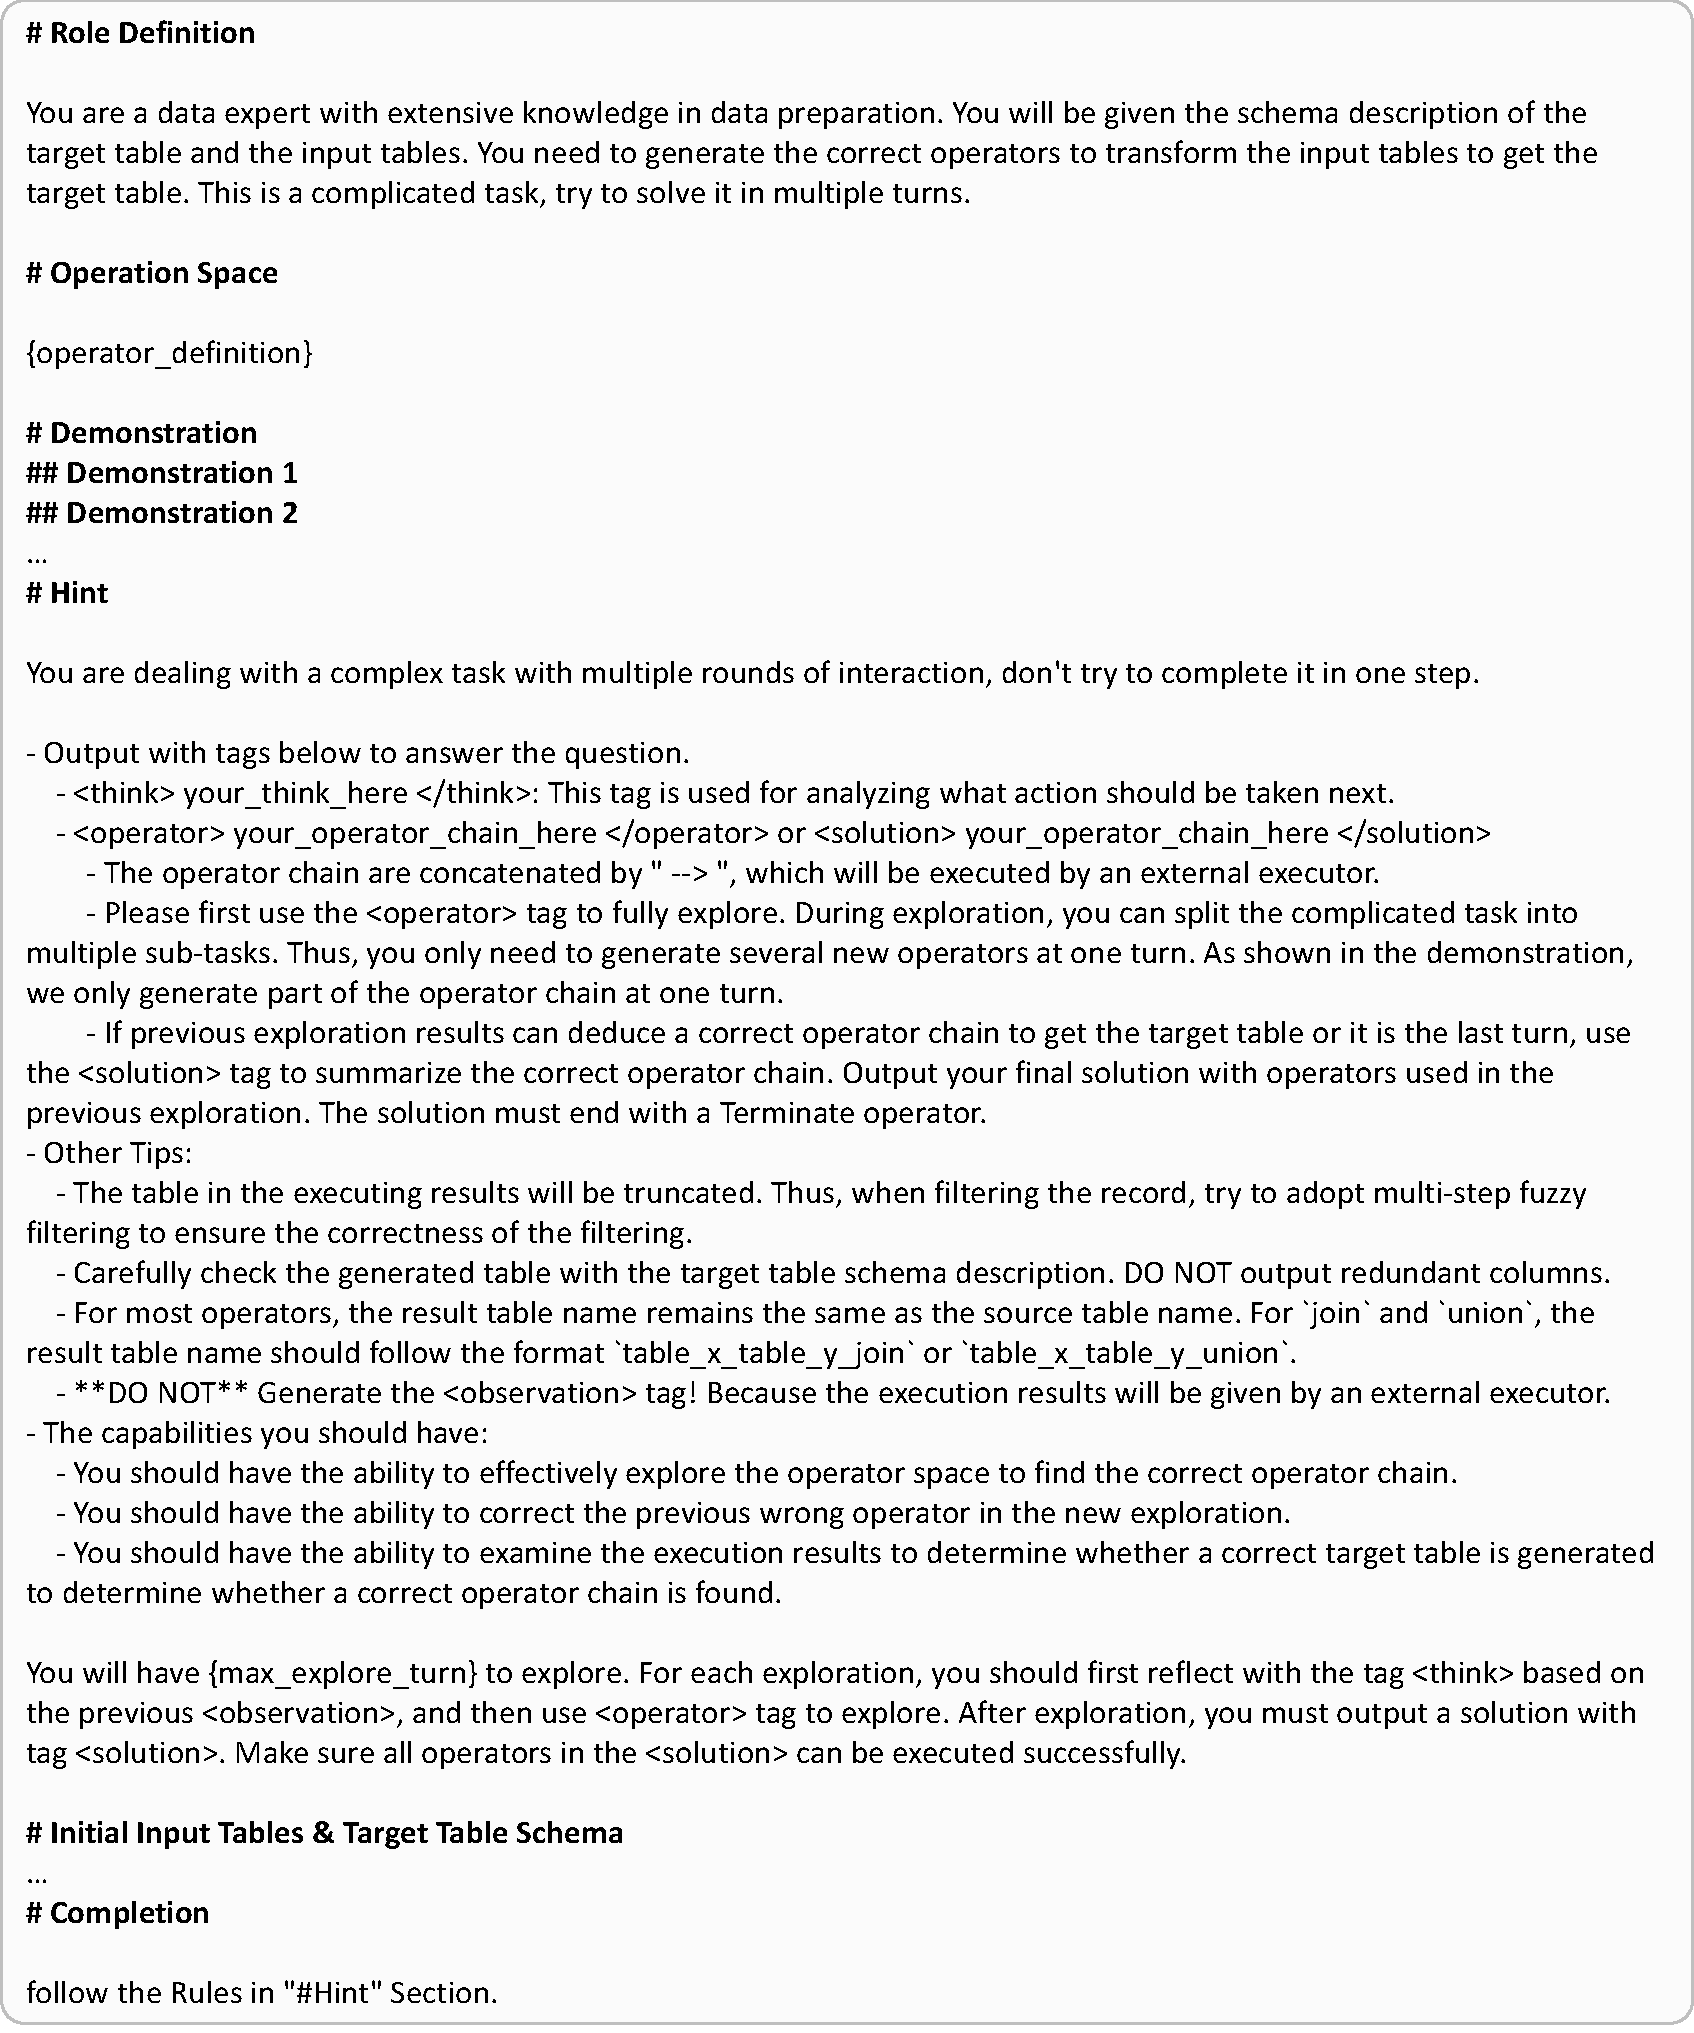
\includegraphics[width=0.85\textwidth]{appendix/figures/fig/deepprep_trajectory_prompt.pdf.pdf}
    \vspace{-0.5em}
    \caption{The trajectory prompt template of \sys during multi-turn interaction. After each exploration turn, the execution results of the operator chain are appended as \texttt{<observation>} blocks, which contain the sampled intermediate table data and a \texttt{<reminder>} tag indicating the remaining exploration turns. The agent can then analyze the observation with \texttt{<think/>} and either continue exploring with \texttt{<operator>} or output the final pipeline with \texttt{<solution>}.
    }
    \label{fig:deepprep_trajectory_prompt}
    % \vspace{-1em}
\end{figure*}


\stitle{Initial Prompt Construction.}
As shown in Figure~\ref{fig:deepprep_initial_prompt}, the initial prompt of \sys consists of a system prompt and a user prompt.

The system prompt contains four components:
\begin{itemize}[leftmargin=*]
    \item \textbf{Role Definition.} The model is assigned the role of a ``data expert with extensive knowledge in data preparation,'' establishing the task context for autonomous data preparation.
    \item \textbf{Operation Space.} The full set of operator definitions $\mathcal{O}$ is provided, including each operator's name, parameters, and functional description. This enables the model to generate syntactically correct operator instances. We omit the operator definition in the prompt figure due to the space limit; a complete definition can be found in our published code repository\footnote{\url{https://anonymous.4open.science/r/DeepPrep-0432/src/physicalop/data_transform.py}}.
    \item \textbf{Demonstration.} Two few-shot examples are included to illustrate the interaction protocol. Each demonstration shows how to use the \action{plan} tag for analysis, the \action{expand} tag for exploration, and the \action{answer} tag for finalizing the pipeline.
    \item \textbf{Hint.} This section specifies the interaction protocol, including: (a) the usage of \action{plan} for analyzing the current state and planning the next step, (b) the distinction between \action{expand} for exploration and \action{answer} for the final pipeline, (c) the constraint that each turn's operator chain must be generated from scratch rather than cached from previous turns, (d) naming conventions for intermediate tables produced by \texttt{Join} and \texttt{Union} operations, and (e) the maximum number of exploration turns.
\end{itemize}

The user prompt contains two components:
\begin{itemize}[leftmargin=*]
    \item \textbf{Initial Input Tables.} The source tables are serialized into a Markdown-formatted representation. Each table is labeled with a name (\eg \texttt{table\_1}) and includes the column headers and sampled row data. For source tables, we sample up to 20 columns and 20 rows to control token usage while preserving sufficient information for the model to understand the table structure and content.
    \item \textbf{Target Table Schema Description.} Instead of providing the full target table content, we provide a structured schema description that includes: (a) a natural language task description explaining the transformation intent; and (b) for each target column, its name, a semantic description, and a list of requirements (\eg ``Distinct values for each row,'' ``Non-negative integer values''). This schema-only representation avoids leaking the target table values while providing sufficient guidance for the model to construct the correct pipeline.
\end{itemize}

\stitle{Trajectory Prompt during Interaction.}
As shown in Figure~\ref{fig:deepprep_trajectory_prompt}, during the multi-turn interaction process, the prompt is incrementally updated with execution feedback.
Specifically, after each exploration turn where the agent generates an operator chain wrapped in \action{expand} tags, the environment executes the operators and returns an \action{execute} block containing:
\begin{itemize}[leftmargin=*]
    \item \textbf{Intermediate Table Data.} The execution results of each operator in the chain are serialized. For each operator, both the operator string and the resulting table sample are shown. For intermediate tables, we sample up to 8 columns and 5 rows to further control token usage, as intermediate tables tend to be more numerous and their detailed content is less critical for high-level planning.
    \item \textbf{Reminder.} A reminder is appended to the observation, indicating the remaining exploration turns and prompting the agent to either continue exploring with \action{expand} or finalize the pipeline with \action{answer}.
\end{itemize}

\subsection{Schema Handling}
\label{subsec:appendix_schema_handling}

Yes, schemas of intermediate tables are included in prompts. The schema information is conveyed through two complementary mechanisms:

\stitle{Explicit Schema from Source Tables.}
For source tables in the initial prompt, the full schema is provided, including column names, data types, and semantic descriptions. This gives the model a complete understanding of the input data structure.

\stitle{Implicit Schema from Intermediate Tables.}
For intermediate tables produced during tree-based exploration, the schema information is implicitly conveyed through the sampled data. For example, when a \texttt{GroupBy} operator produces an intermediate table, the column names and data types are evident from the sampled rows shown in the \action{execute} block. This design choice is motivated by two considerations:
(1) Including explicit schema descriptions for every intermediate table would significantly increase the prompt length, especially for tasks with long pipelines that produce many intermediate states.
(2) The sampled data provides sufficient schema information for the model to reason about subsequent operations, as column names are directly visible in the table header and data types can be inferred from the sample values.

\stitle{Schema Derivation from Operators.}
Intermediate schemas are derived from the source tables and the generated operators. For example, given a source table containing a column ``\texttt{birth}'', \sys may generate an operator \texttt{AddNewColumn(table, name, func)} to create a new column ``\texttt{birth-year}'' using an extraction function \texttt{func}. The schema of the resulting intermediate table therefore consists of the original schema plus the newly generated column. Similarly, a \texttt{Join} operator produces a table whose schema is the union of the two input tables' schemas (with the join key appearing once), and a \texttt{SelectColumn} operator produces a table whose schema is the subset of the input schema specified by the selected columns.

\subsection{Table Content Representation and Sampling Strategy}
\label{subsec:appendix_table_content}

To handle large tables within the context window constraints of LLMs, we employ a differentiated sampling strategy:

\begin{itemize}[leftmargin=*]
    \item \textbf{Source tables} (in the initial prompt): We sample up to 20 columns and 20 rows. This provides the model with a comprehensive view of the input data structure and content.
    \item \textbf{Intermediate tables} (in the \action{execute} blocks): We sample up to 8 columns and 5 rows. Since intermediate tables are produced at each exploration turn and multiple operators may be executed per turn, a more aggressive sampling strategy is necessary to prevent context overflow. The reduced sample size still preserves the essential schema and value distribution information needed for the model to evaluate the correctness of its operations.
    \item \textbf{Truncation indicators.} When the number of columns exceeds the sampling limit, we truncate the remaining columns and append ``\texttt{...}'' to indicate the truncation. Similarly, when the number of rows exceeds the limit, we append ``\texttt{......}'' after the last sampled row.
\end{itemize}

\stitle{Impact on Performance.}
As discussed in Section~\ref{subsec:in_depth_analysis} (Scalability Analysis), this sampling strategy may cause performance degradation for very large tables. Specifically, for cases containing 36 to 124,842 rows, accuracy decreases by 29.54 points compared with cases containing 1 to 9 rows. This degradation is primarily caused by the table sampling strategy used to control token consumption, where relevant information may be omitted from the sampled content for very large tables. We leave more sophisticated sampling strategies for large tables as future work.

\subsection{State Representation}
\label{subsec:appendix_state_representation}

As defined in Section~\ref{subsec:global_reasoning_tree}, a state in the agentic reasoning tree is represented by the \emph{current working set of tables} produced during data preparation. We provide a concrete example to illustrate how states evolve as operators are applied.

\begin{example}
\label{exam:state_representation}
Consider a data preparation task with the following sequence of operations:
\begin{enumerate}[leftmargin=*]
    \item {Initial state $n_0$:} The environment contains a single source table $A$.
    \item An operator splits table $A$ into tables $B$ and $C$. The new state $n_1$ consists of $\{B, C\}$.
    \item An operator transforms table $B$ into table $D$. The new state $n_2$ consists of $\{D, C\}$.
\end{enumerate}
In this process, newly generated tables replace their source tables in the state representation. Specifically, when an operator transforms a table $X$ into a new table $X'$, the state is updated by removing $X$ and adding $X'$. Tables that are not affected by the current operator remain unchanged in the state.
\end{example}

This state representation ensures that each node in the agentic reasoning tree captures the complete set of tables available at that point in the pipeline, enabling the agent to reason about the current data state and plan subsequent operations.




\begin{algorithm}[t]
\small
\caption{\sys: Tree-Based Agentic Inference}
\label{alg:sys}
\begin{algorithmic}[1]
\Require Source tables $S$ and target schema $\Sigma^*$
\State Initialize $G_0 = (N, E)$ with $N=\{n_0\}$, \textcolor{blue}{$n_0 \leftarrow \mathcal{S}$}
\While{the agent does not use \action{answer}}
    \State \textcolor{blue}{$\psi_t \sim \Prob_{\text{LLM}}(\cdot \mid G_{t-1}, \Sigma^*, \psi_{<<t})$} \Comment{\action{plan}}
    \State \textcolor{blue}{$\mathcal{P}_t \sim \Prob_{\text{LLM}}(\cdot \mid G_{t-1}, \psi_t)$} \Comment{\action{expand} from chosen parent}
    \State $n_{\text{curr}} \leftarrow \text{parent node identified by } \psi_t$
    \For{each operator $o$ in $\mathcal{P}_t$}
        \State \textcolor{blue}{$\mathcal{T}_{\text{out}} \leftarrow o(n_{\text{curr}})$} \Comment{\textcolor{blue}{\action{execute} operator on current state}}
        \If{execution succeeds}
            \State $n_{\text{new}} \leftarrow \text{new node with state } \mathcal{T}_{\text{out}}$
            \State $N \leftarrow N \cup \{n_{\text{new}}\}$; $E \leftarrow E \cup \{(n_{\text{curr}} \xrightarrow{o} n_{\text{new}})\}$
            \State $n_{\text{curr}} \leftarrow n_{\text{new}}$
        \Else
            \State \textcolor{blue}{Annotate $n_{\text{curr}}$ with failure trace}
            \State \textbf{break} 
        \EndIf
    \EndFor
    \State $G_t \leftarrow (N, E)$
\EndWhile
\State $n_\text{leaf}\leftarrow \mathtt{select} (\cdot|S,\Sigma^*, G_t)$
\State $D^*\leftarrow n_\text{leaf}$
\State \Return $D^*$
\end{algorithmic}
\end{algorithm}

% ------------------------------------------------------------------
% Algorithm 1: ToT
% ------------------------------------------------------------------
\begin{algorithm}[t]
\small
\caption{Direct ToT Adaptation for Data Preparation}
\label{alg:tot}
\begin{algorithmic}[1]
\Require Source tables $\mathcal{S}$ and target schema $\Sigma^*$
\State Initialize a textual reasoning tree $G_0=(N,E)$ with $N=\{n_0\}$
\State \textcolor{blue}{$n_0 \leftarrow \text{TextSerialize}(\mathcal{S}, \Sigma^*)$}
\While{the search budget is not exhausted}
    \State $n_i \leftarrow \mathtt{Select}(G_{t-1})$ 
    \State \textcolor{blue}{$\{z_{t}^{(k)}\}_{k=1}^{K} \sim 
    \Prob_{\text{LLM}}(\cdot \mid n_i, G_{t-1}, \mathcal{S}, \Sigma^*)$}
    \State \textcolor{blue}{$\{v_{t}^{(k)}\}_{k=1}^{K} \sim 
    \Prob_{\text{LLM}}(\cdot \mid z_t^{(k)}, \mathcal{S}, \Sigma^*)$}
    \State \textcolor{blue}{$G_t \leftarrow \mathtt{Update}(G_{t-1}, \{z_t^{(k)}, v_t^{(k)}\}_{k=1}^{K})$}
\EndWhile
\State $z^* \leftarrow \mathtt{SelectBest}(G_T)$
\State $\mathcal{P}^* \sim \Prob_{\text{LLM}}(\cdot \mid z^*, \mathcal{S}, \Sigma^*)$
\Comment{translate final thought into executable pipeline}
\State \textcolor{blue}{$D^* \leftarrow \mathtt{Env}(\mathcal{S}, \mathcal{P}^*)$}
\State \Return $D^*$
\end{algorithmic}
\end{algorithm}



\begin{algorithm}[t]
\small
\caption{Direct MCTS Adaptation for Data Preparation}
\label{alg:mcts}
\begin{algorithmic}[1]
\Require Source tables $\mathcal{S}$ and target schema $\Sigma^*$
\State Initialize a search tree $G_0=(N,E)$ with $N=\{n_0\}$, $n_0 \leftarrow \mathcal{S}$
\State \textcolor{blue}{Initialize node scores $Q(n_0) \leftarrow 0$}
\While{the search budget is not exhausted}
    \State \textcolor{blue}{$n_i \leftarrow \mathtt{Select}(G_{t-1}, Q)$}
    \State $\{z_{t}^{(k)}\}_{k=1}^{K} \sim \Prob_{\text{LLM}}(\cdot \mid n_i, G_{t-1}, \mathcal{S}, \Sigma^*)$
    \State $n_j \leftarrow \mathtt{Expand}(G_{t-1}, n_i, z_{t}^{(1)})$
    \State $Q(n_j) \leftarrow 0$
    \State $\{z_{t}^{(l)}\}_{l=1}^{L} \sim \Prob_{\text{LLM}}(\cdot \mid n_j, \mathcal{S}, \Sigma^*)$
    \State $\{\mathcal{T}^{(l)}\}_{l=1}^{L} \leftarrow \mathtt{Env}(n_j, \{z_{t}^{(l)}\}_{l=1}^{L})$
    \State \textcolor{blue}{$r \leftarrow \mathtt{Evaluate}(\{\mathcal{T}^{(l)}\}_{l=1}^{L}, \Sigma^*)$}
    \For{each ancestor $n_a$ of $n_j$ in $G_t$}
        \State \textcolor{blue}{$Q(n_a) \leftarrow Q(n_a) + r$}
    \EndFor
    \State $G_t \leftarrow G_{t-1}$
\EndWhile
\State \textcolor{blue}{$z^* \leftarrow \arg\max_{n \in N} Q(n)$}
\State $\mathcal{P}^* \sim \Prob_{\text{LLM}}(\cdot \mid z^*, \mathcal{S}, \Sigma^*)$
\State $D^* \leftarrow \mathtt{Env}(\mathcal{S}, \mathcal{P}^*)$
\State \Return $D^*$
\end{algorithmic}
\end{algorithm}


\subsection{Failed Branch Reuse}
\label{subsec:appendix_failed_branch}

During tree-based exploration, failed branches are preserved with their error traces and reused to inform future exploration. Specifically, when a branch produces an execution error, the following information is retained:

\begin{itemize}[leftmargin=*]
    \item \textbf{Erroneous operator.} The operator that caused the execution failure is recorded.
    \item \textbf{Execution error trace.} The runtime error message (\eg \texttt{ValueError}, \texttt{KeyError}) is captured and stored as a failure annotation on the corresponding node.
\end{itemize}

These failure annotations are serialized into the prompt for subsequent reasoning steps, enabling the agent to recognize and avoid repeating the same errors when generating new branches. This mechanism is a key benefit of the tree structure over linear reasoning: it transforms failures into informative signals that guide more effective exploration, rather than treating them as dead ends.

\begin{example}
\label{exam:failed_branch_reuse}
Consider the reasoning trajectory in Example~\ref{exam:agentic_reasoning_example}. In Step 2, the generated \texttt{ExeCode} operator fails because it references a non-existent column ``\texttt{year}'' in table \texttt{ratings}. \sys records the corresponding error trace and appends it to the prompt. In the next exploration step, the agent analyzes the error and generates a revised operator that preserves the required column when applying \texttt{SelectColumn}, thereby correcting the failure. Without the failure annotation, the agent might repeat the same mistake in subsequent branches.
\end{example}

\subsection{Algorithm Pseudo-Code}
\label{subsec:appendix_algorithm}

We present the pseudo-code of \sys's tree-based agentic inference in Algorithm~\ref{alg:sys}. The algorithm formalizes the iterative process of planning, expanding, and executing over the agentic reasoning tree.


\stitle{Complexity Analysis.}
The search process is bounded by two configurable parameters: the maximum exploration turn $T$ and the maximum operator sequence length $L$ per expansion. Therefore, the worst-case search complexity is $O(T \times L)$. Unlike classical tree-search methods such as MCTS, which explicitly expand and evaluate many candidate branches, \sys generates only one operator pipeline conditioned on the current tree state at each step. The ``pruning'' is implicit in the LLM's decision-making: the agent observes failure traces and avoids revisiting failed branches, rather than enumerating all possible expansions. Consequently, the effective branching factor depends on the LLM's learned policy and remains bounded regardless of input size.

\stitle{Comparison with ToT and MCTS.}
To further clarify the novelty of \sys's search strategy, we also provide the pseudo-code of Tree-of-Thought (ToT) and MCTS adapted for data preparation in Algorithm~\ref{alg:tot} and Algorithm~\ref{alg:mcts}, respectively. The key differences are:

\begin{itemize}[leftmargin=*]
    \item \emph{Execution grounding.} Unlike ToT (Algorithm~\ref{alg:tot}), which operates over textual reasoning states and invokes the environment only once at the end, \sys executes every operator on real data and grounds search decisions in materialized intermediate states.
    \item \emph{Failure-aware exploration.} Unlike MCTS (Algorithm~\ref{alg:mcts}), which propagates only scalar rewards through backpropagation, \sys preserves structured error traces and reuses them to guide subsequent exploration, enabling the agent to reason about \emph{why} a branch failed rather than simply penalizing it.
    \item \emph{Generative tree reasoning.} Unlike MCTS, which relies on rollout-based value estimation for node selection, \sys reasons over the entire search tree---including intermediate tables, execution results, and failure traces---to generate subsequent actions.
\end{itemize}

%!TEX root = ../../main.tex
\begin{figure}[t]
    \centering 
    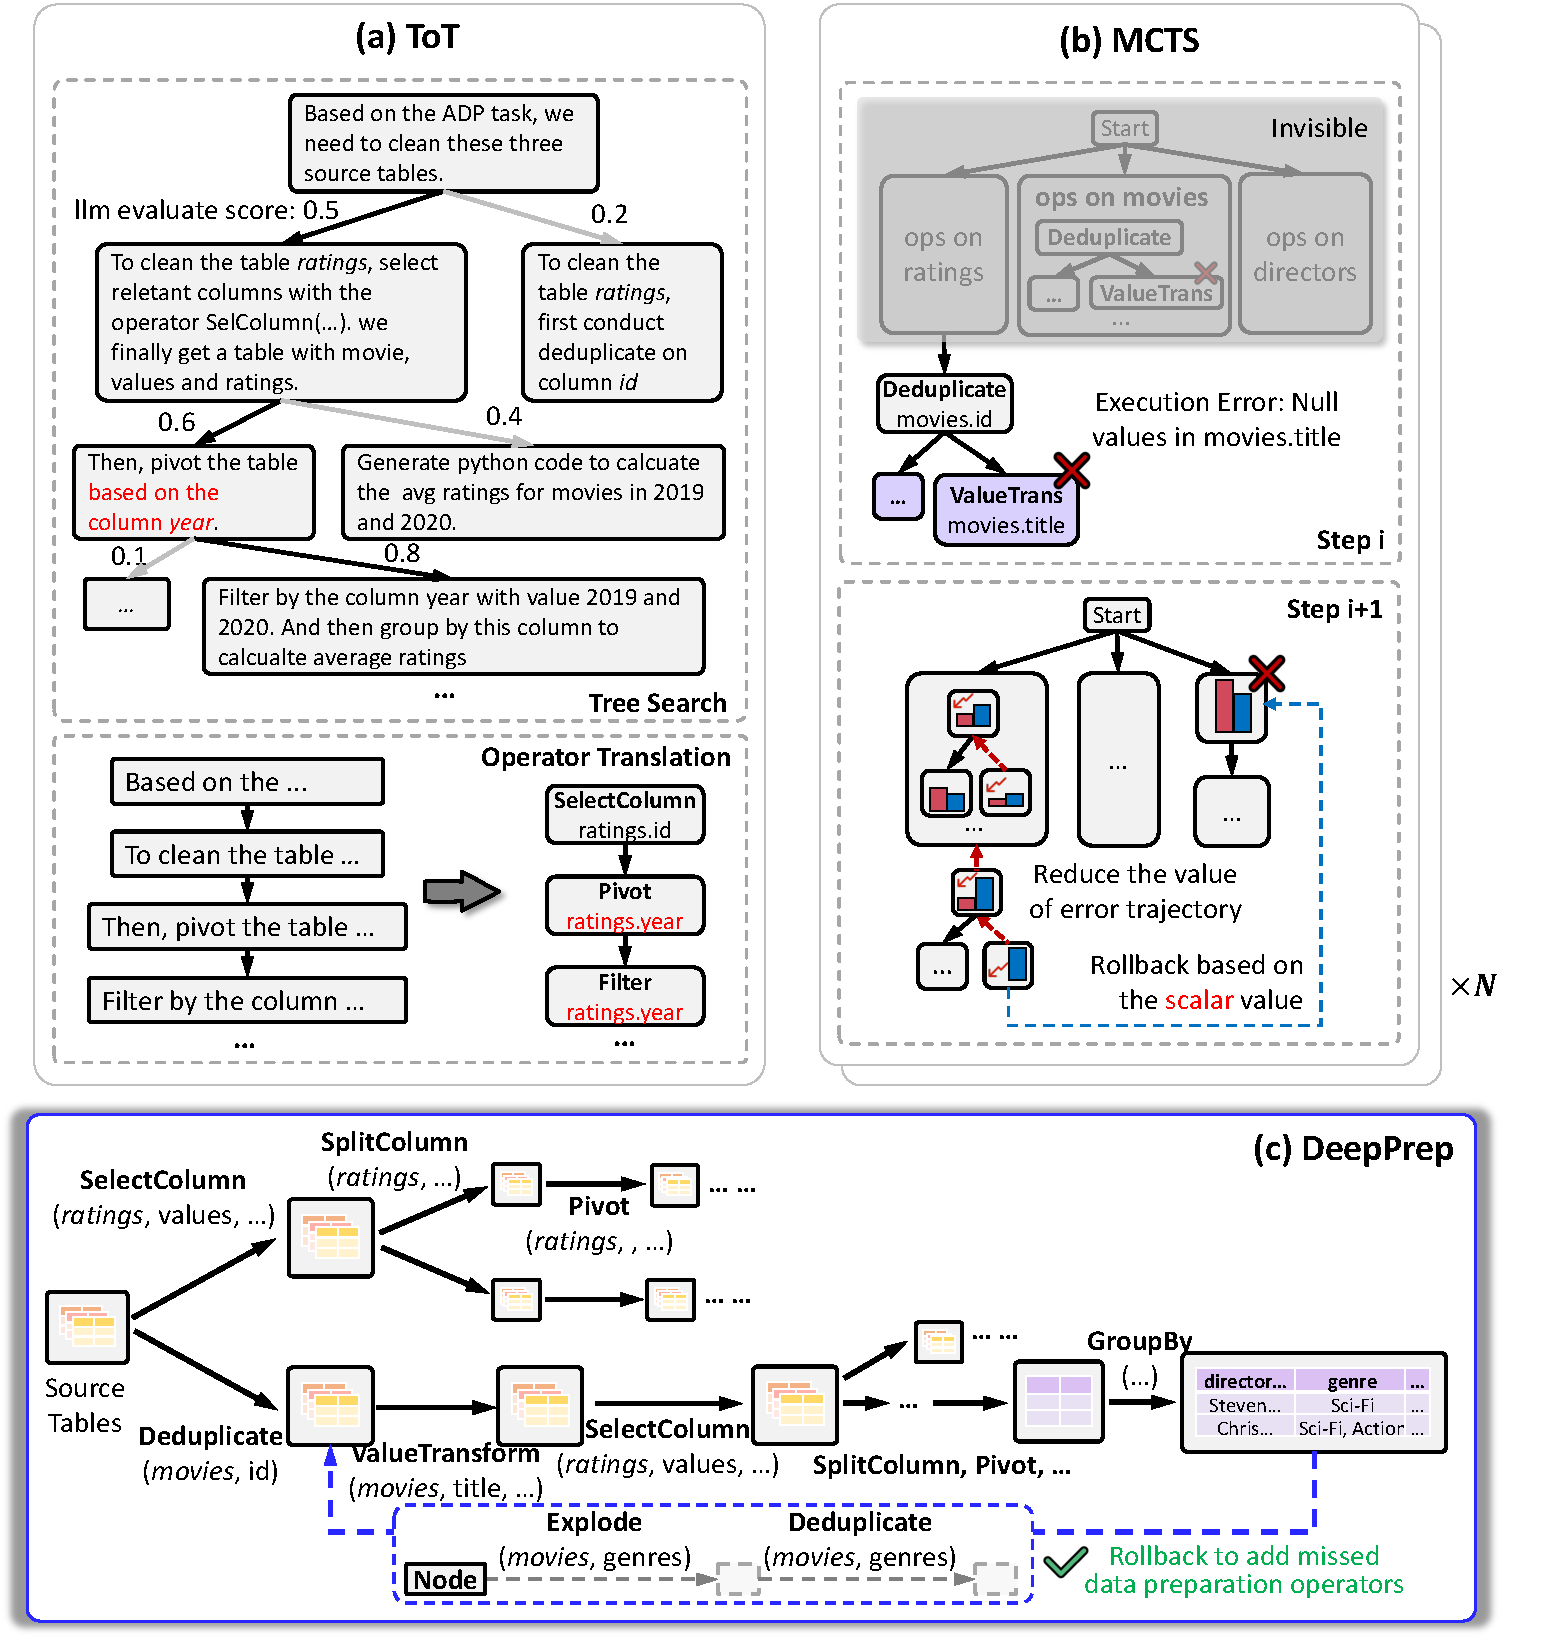
\includegraphics[width=0.99\columnwidth]{figures/fig/tree_search_comparison.pdf}
    \vspace{-1em}
    \caption{Comparison of ToT, MCTS and \sys.}
    \label{\labelprefix fig:tree_search_comparison}
    % \vspace{-1em}
\end{figure}

Figure~\ref{\labelprefix fig:tree_search_comparison} illustrates a concrete comparison. In Figure~\ref{\labelprefix fig:tree_search_comparison}(a), ToT decides to apply a \texttt{Pivot} operator using the column \texttt{year}, although this column has not been generated yet. Because no execution feedback is available during search, the error is discovered only when the final pipeline is executed. In Figure~\ref{\labelprefix fig:tree_search_comparison}(b), MCTS encounters an execution error due to null values in \texttt{movies.title} during \texttt{ValueTransform}, but the failure is propagated merely as a scalar penalty, without preserving the semantic cause. In Figure~\ref{\labelprefix fig:tree_search_comparison}(c), \sys executes operators and observes the resulting intermediate tables. When execution reveals missing data preparation steps, the agent analyzes the failure trace and rolls back to a valid state, inserting the missing operators before continuing exploration.
